\chapter{Motivation and overview aboard the thesis}
\label{chap:outline}

\section{Motivation of Thesis}
Since 2014, Tesla CEO Elon Musk has made a lot of promises about self-driving cars being less than a year away \cite{tangermann-2022}. While one can admire his enthusiasm and optimism, he has not yet fulfilled this promise and a full self-driving car is yet to be made. In July 2021 Musk admitted in a tweet that \textit{"(...) Generalized self-driving is a hard problem, as it requires solving a large part of real-world AI. Didn’t expect it to be so hard, but the difficulty is obvious in retrospect.  Nothing has more degrees of freedom than reality."} \cite{musk-2021}. \bigskip

When talking about autonomous driving, SAE International defined 5 levels of automation:
\begin{enumerate}
    \item [Level 0] The human driver does everything.
    \item [Level 1] An automated system can assist the human driver in conducting one part of the driving task for extended periods.
    \item [Level 2] An automated system can assist the driver with multiple parts of the driving task for extended periods. The driver must continue to monitor the driving environment and be actively engaged.
    \item [Level 3] An automated system conducts all of the driving task without driver engagement and monitors the driving environment, but the human driver must stand by to intervene in response to a system failure or request from the system to take over.
    \item [Level 4] An automated system can conduct the entire driving task without driver input but only in certain conditions (e.g., limited to 25 mph) or places (e.g., a city center).
    \item [Level 5] An automated system can perform the entire driving task without driver input under all conditions.
\end{enumerate}
For now, we still have to drive or own car although we already use advanced driver assistance \cite{insurance-institute-for-highway-safety-2022}. To get to Level 5, there is still a lot of research to be done.\bigskip

An important component of a self-driving car is environment perception. In this thesis, I will investigate how information about the geometrical environment of the racing car can be obtained from visual image sequences. Of course, given the short time span I have to work on this thesis, I will not be able to manage a full working solution. With this thesis, I aim to lay the groundwork of this environment perception.

\subsection{Personal Motivation}
In the process of looking for a subject to write my masters thesis about, my supervisor professor Rudolf Mester and I were talking about the different possibilities in the field of computer vision. I am very much interested in car racing, and that is how we stumbled upon Revolve NTNU, a group of students that take part in the Formula Student competitions \cite{unknown-author-no-date}.\bigskip

One of the challenges they have to tackle is a driverless competition. So far, they have used a LiDAR sensor (light detection and ranging) to estimate the position and movements of the car as well as the cones that mark the drivable area. Another way to do this is by using camera footage and computer vision. As a LiDAR sensor is quite costly in comparison to a simple camera, this is a cheaper solution. That is provided of real-time interpretation of the video signal can be solved. In this thesis, I will address this. As stated before the overall problem is too big to be solved in a single Masters thesis project, so this thesis shall provide some essential elements for such a visual perception approach.\bigskip

\section{Objectives of thesis}
\subsection{Primary objectives}
My goal is to lay down the basic work for Revolve NTNU to help them change their approach to this challenge. To do this, I will try to build a computer vision software system that is able to extract the motion of a moving car to the extent possible in the course of a master thesis. \bigskip

I will work with footage from the racing car that Revolve NTNU shot in previous competitions. \autoref{fig:footage} is a frame of this footage. As you can see, the camera is attached to the side of the car and mounted slightly tilted. The racing tracks they race on are marked by cones and a thin white line. The road surface they race on will be considered a (more or less) flat surface.\bigskip

\begin{figure}
    \centering
    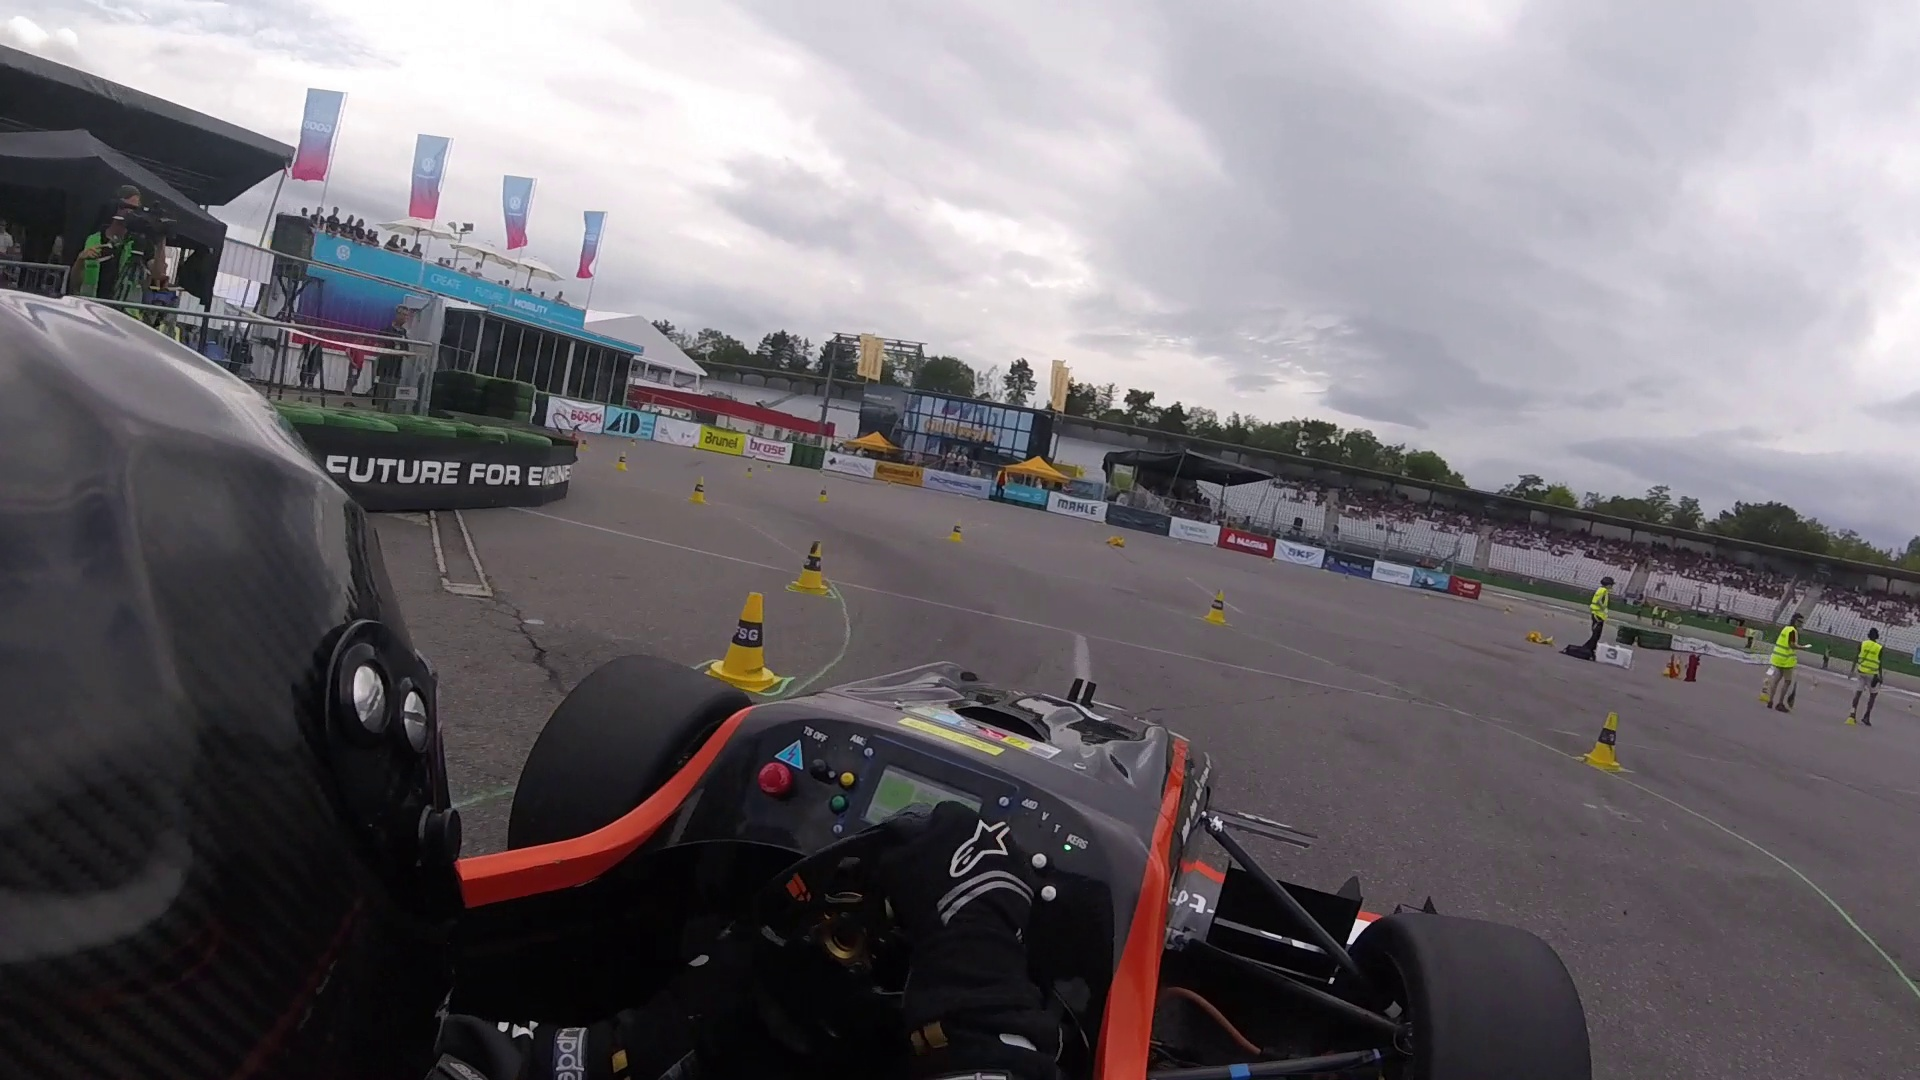
\includegraphics[width=1\textwidth]{figures/footage_example.jpg}
    \caption{Example of footage}
    \label{fig:footage}
\end{figure}

The software system should be able to do the following:
\begin{itemize}
    \item Estimate the frame-to-frame motion of a racing car and the momentary orientation of the camera with respect to the ground plane.
    \item Create a birds eye view map of the environment  that is in front of the car at any time, in particular the positions of the cones which are used to mark the drivable path.
\end{itemize}

\subsection{Secondary objectives}
Based on the previous features of the system, two additional features could be added: 
\begin{itemize}
    \item Reconstruction of the car's trajectory over time.
    \item Building a global map from the instantaneous map.
\end{itemize}

\subsection{Future goals}
I will of course not be able to build a whole system that is able to let a car drive autonomously starting from scratch. I will lay the groundwork upon which can be built. Using these solutions to the previous stated problems, the system could be expanded and obstacles, side barriers etc. could be entered into the map previously mentioned.


\section{Determining motion from a set of point correspondences}\label{sec:determmot}
We now have a way to describe motion in the form of a rotation matrix and a translation vector. To determine this motion, we need to have some corresponding points from each pose. Assuming we have these (I will discuss how to get these in detail later on) there are two cases, the general case where the keypoints can not all lie in one plane. However if this is the case, there's a second option to handle this. The difficulty in all this is that we are working with images, which are 2-D representations of a 3-D world. 


\section{Point-to-point correspondences}
In \autoref{sec:determmot} we talked about the need for point correspondences in consecutive frames to estimate either the essential or homography matrix in order to determine motion.\bigskip

\subsection{Local image features}
To look for point correspondences, we first need to look for recognisable points. A local image feature describes a small region of an image. It consists of a keypoint, which is the image coordinate of the image patch and a descriptor which describes the content of that patch.\bigskip

Using a keypoint detector it is possible to find keypoints in an image. Keypoint description methods make it possible to describe the patch and compare keypoints across different images. In section \autoref{sec:keydet} we describe these in detail as well as the used keypoint detector and description methods.

\section{Contributions of this thesis}

\section{Overview of the Thesis}
This thesis consists of 6 chapters. \autoref{chap:outline} gives a brief introduction to the thesis together with an overview in what has been accomplished. In \autoref{chap:theoretic_found} I explain the theoretical foundation of geometrical computer vision that is needed to understand the thesis. In \autoref{chap:found_mot_est} do the same for image analysis for motion estimation.\bigskip

I discuss the steps I took in building the software system in \autoref{chap:system_implementation}. \autoref{chap:exp_results} gives an overview of the experiments and their results that have been conducted. I conclude this thesis in \autoref{chap:conclusion} with a summary and conclusion.
